%%%%%%%%%%%%%%%%%%%%%%%%%%%%%%%%%%%%%%%%%%%%%%%%%%%%%%%%%%%%%%%%%%%%%%%
 \input texbas.inp
%======================================================================
 \documentclass[11pt]{article} % ,a4paper ,fleqn
%======================================================================
 \usepackage{tikz}
 \usepackage{pgfplots}
 \pgfplotsset{compat=1.17}
%======================================================================
 \usepackage[english]{babel}
% \usepackage[dutch]{babel}
 \usepackage{a4wide}
 \usepackage{longtable}
 \usepackage{epic,eepic}
 \usepackage{epsf}
 \usepackage{epsfig}
 \usepackage{psfrag}
 \usepackage{exscale}
 \usepackage{amssymb}
 \usepackage{euler}
% \usepackage{pstricks}
% \usepackage{rotating}                  
 \usepackage{alltt}
 \usepackage{verbatim}
% \usepackage[usenames]{color}
% \usepackage{listings,comment}
% \excludecomment{listing}
% \usepackage[urlcolor=blue,colorlinks=true]{hyperref}
%======================================================================
% \usepackage{hyperref}
% \hypersetup{ bookmarks = false
%            ,pdftitle = {educational stuff}
%            ,pdfborderstyle = {/S/U/W 1} % {/S/U} % 
%            ,pdfborder = 0 0 0 
%            ,colorlinks = true
%            ,linkbordercolor = red
%            ,linkcolor = blue
%            ,citecolor = blue
%            ,urlcolor = blue
%            ,linktoc = page
% }
%======================================================================
\begin{document}
%======================================================================
 \newlength{\figscale}
 \setlength{\figscale}{0.001in}
 \newcommand{\picfontsize}{\normalsize}
 \newcommand{\FIG}[3]{%
 \setlength{\unitlength}{#1#2}\mbox{} 
 \begin{center} {\picfontsize #3 } \end{center}\mbox{}}
 \newcommand{\FIGDIR}{\MYTEXDIR/../tpl}
%========================================
 \setlength{\parindent}{0em}
 \pagenumbering{arabic} 
% \pagenumbering{Roman}
 \pagestyle{empty}
% \pagestyle{myheadings}
% \setcounter{page}{0}
% \setcounter{fignum}{0}
%======================================================================

The next {\color{red}figure} is {\bf test-eepic.eepic}.
It is made with {\em xfig} and exported to .eepic format.
\\

\FIG{0.5}{\figscale}{\input \FIGDIR/test-eepic.eepic}

The next {\color{red}figure} is {\bf test-eps1.eps}.
This is also made with {\em xfig} and exported to .eps format.
Package {\em psfrag} is used to place text in the figure.
\\

\begin{center}
\psfragscanon
\psfrag{$\frac{1}{2}$}[bc][bc]{text 1}
\psfrag{text}[tc][tc]{text 2}
\psfrag{$\frac{1}{2}$}[lc][lc]{\Large text 3}
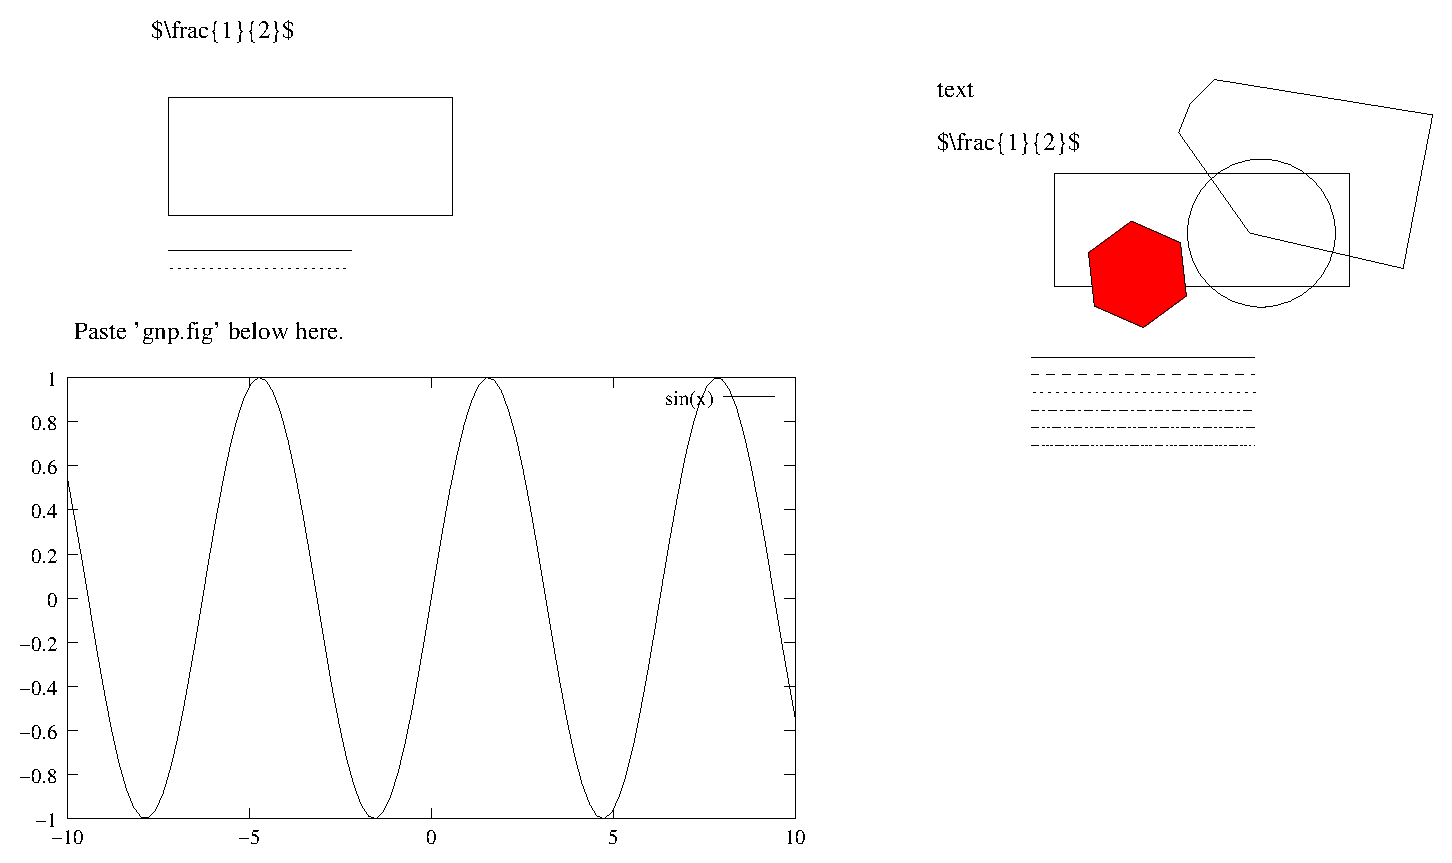
\includegraphics[width=0.7\textwidth]{\FIGDIR/test-eps1.eps}
\psfragscanoff
\end{center}

%======================================================================
\newpage

The {\color{red}figure} below is {\bf test-eps2.eps} and made 
with {\em Matlab}.
Package {\em psfrag} is used to place text in the figure.
\\

\psfragscanon
\psfrag{xl}[tc][tc]{\fbox{xlabel}}
\psfrag{yl}[rc][tc]{\fbox{ylabel}}
\psfrag{tl}[bc][lc]{\fbox{title}}
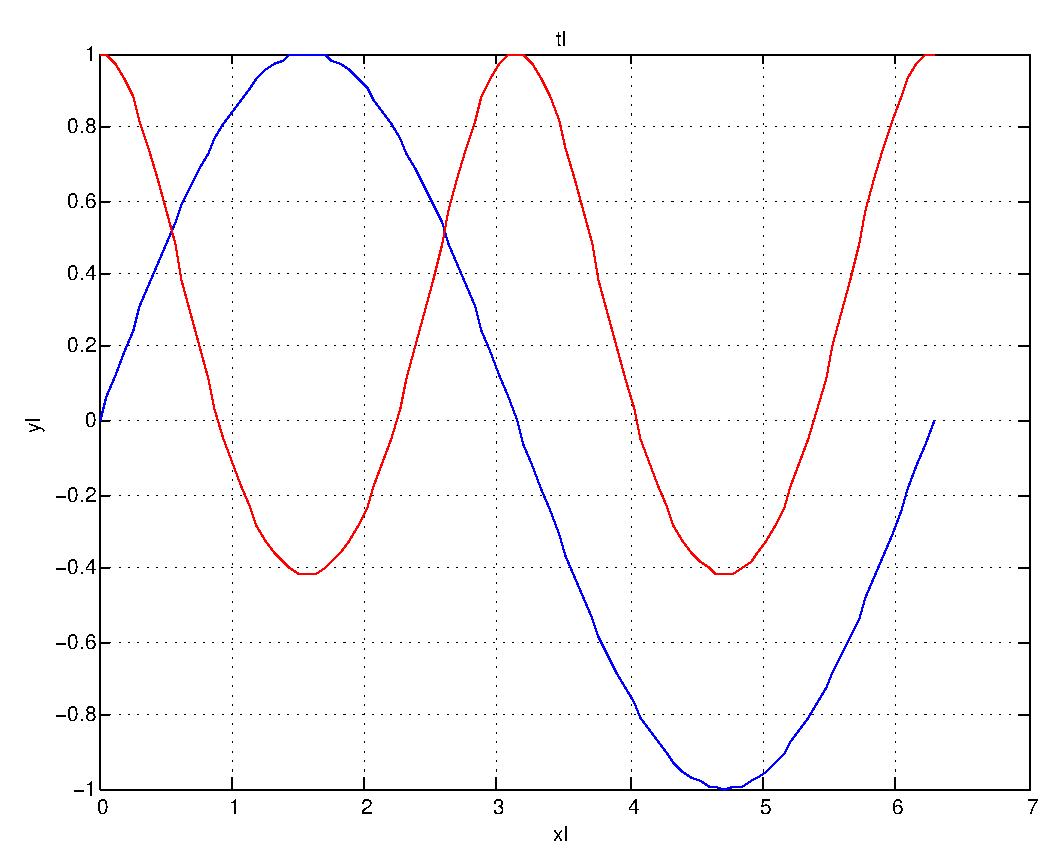
\includegraphics[width=90mm]{\FIGDIR/test-eps2.eps}
\psfragscanoff

~\\

Formulas are typeset in {\bf euler} font~:

\[
   y = \sqrt{\frac{\sin(\alpha)}{\cos(\varepsilon)}}
   \hspace*{5mm};\hspace*{5mm}
   \mbox{\boldmath $\sigma$}_{ij} = 
   \int\limits_{x=0}^{x=\infty} 
   {^4 \mbox{\boldmath $M$}} : \mbox{\boldmath $\varepsilon$} \, dx
\]

%======================================================================
\newpage

Ths is an eepic file generated with gnuplot.
\\

\input \FIGDIR/test-gnp.tex

\newpage

An external text-file can be included with {\em verbatiminput}.

\verbatiminput{\FIGDIR/test-txt1.txt}

%======================================================================
\newpage

Basic plotting can be done with {\em pgfplots}.
\\

\begin{tikzpicture}
  \begin{axis}
    \addplot[color=red]{exp(x)};
  \end{axis}
\end{tikzpicture}

%======================================================================
\end{document}
%%%%%%%%%%%%%%%%%%%%%%%%%%%%%%%%%%%%%%%%%%%%%%%%%%%%%%%%%%%%%%%%%%%%%%%
